\documentclass[12pt,fleqn]{examtst}
\usepackage{graphicx}
\usepackage{amssymb}
\usepackage{amsmath}
\usepackage{listings}
\usepackage{multirow}
\usepackage{multicol}
\usepackage{hhline}
\usepackage{booktabs}
\usepackage{url}
\usepackage{enumerate}
\usepackage{hyperref}
%% Comments

\usepackage{color}

\newif\ifcomments\commentstrue

\ifcomments
\newcommand{\authornote}[3]{\textcolor{#1}{[#3 ---#2]}}
\newcommand{\todo}[1]{\textcolor{red}{[TODO: #1]}}
\else
\newcommand{\authornote}[3]{}
\newcommand{\todo}[1]{}
\fi

\newcommand{\wss}[1]{\authornote{blue}{SS}{#1}}

\begin{document}

\newcommand{\soln}{n} %y for yes and n for no

\lstset{language=python, basicstyle=\ttfamily, breaklines=true,
  showspaces=false, showstringspaces=false, breakatwhitespace=true}

\newcommand{\codeit}[1]{\texttt{\textit{#1}}}

\begin{center}
  {\large \bf COMP SCI 2ME3 and SFWR ENG 2AA4 Midterm Examination}\\[1ex]
  {\large \bf McMaster University}\\[1ex]
  \ifthenelse{\equal{\soln}{y}}{\large {\bf ANSWER KEY} %Large arrow
    %($\Longleftarrow$) for correct% , small ($\leftarrow$) for partially
    % correct
  }{}
\end{center}

\medskip

\noindent
DAY CLASS%, \textbf{Version 1}
\hfill Dr.~S.~Smith \\
DURATION OF EXAMINATION: 3 hours \\
MCMASTER UNIVERSITY MIDTERM EXAMINATION \hfill March 4, 2021

\medskip

\noindent
\rule[3 mm]{\textwidth}{0.5mm}

%\begin{minipage}[t]{1.0\textwidth}

NAME: \wss{Enter your name here}\\[1ex]

Student ID: \wss{Enter your student number here} \\[2mm]

\noindent
\rule[3 mm]{\textwidth}{0.5mm}

This examination paper includes \noofpages pages and
4 % VARIABILITY
questions. You are responsible for ensuring that your copy of the examination
paper is complete. Bring any discrepancy to the attention
of your instructor.\\

\noindent
\emph{By submitting this work, I certify that the work represents solely my own
independent efforts. I confirm that I am expected to exhibit honesty and use
ethical behaviour in all aspects of the learning process.  I confirm that it is
my responsibility to understand what constitutes academic dishonesty under the
\href{https://secretariat.mcmaster.ca/app/uploads/Academic-Integrity-Policy-1-1.pdf}
{Academic Integrity Policy}}.\\

\noindent
\textbf{Special Instructions}:

\begin{enumerate}

\item For taking tests remotely: 
\begin{itemize}
\item Turn off all unnecessary programs, especially Netflix, YouTube, games like
  Xbox or PS4, anything that might be downloading or streaming.
\item If your house is shared, ask others to refrain from doing those activities
  during the test.
\item If you can, connect to the internet via a wired connection.
\item Move close to the Wi-Fi hub in your house. 
\item Restart your computer, 1-2 hours before the exam. A restart can be very
  helpful for several computer hiccups.
\item Commit and push your tex file, compiled pdf file, and code files
  frequently.
\item Ensure that you push your solution (tex file, pdf file and code files)
  before time expires on the test.  The solution that is in the repo at the
  deadline is the solution that will be graded.
\end{itemize}
\item It is your responsibility to ensure that the answer sheet is properly
  completed. Your examination result depends upon proper attention to the
  instructions.
\item All physical external resources are permitted, including textbooks, calculators,
  computers, compilers, and the internet.
\item The work has to be completed individually.  Discussion with others is
  strictly prohibited.
\item Read each question carefully.
\item Try to allocate your time sensibly and divide it appropriately between the
  questions.
\item The set $\mathbb{N}$ is assumed to include $0$.
\end{enumerate}
%\end{minipage}\\

\examheader{CS2ME3/SE2AA4 \ifthenelse{\equal{\soln}{y}} {\hfill SOLUTIONS} }

\renewcommand{\labelenumi}{\Alph{enumi}.}

\newpage

%%%%%%%%%%%%%%%%%%%%%%%%%%%%%%%%%%%%%%%%%%%%%%%%%%%%%%%%%%%%%%%%%%%%%%

\question{6 marks} %tests software qualities - reusability?
Parnas advocates faking a rational design process as depicted in the figure below.
The faked documentation follows these steps: Requirements (SRS) $\rightarrow$
Design (MG and MIS) $\rightarrow$ Application Implementation (code)
$\rightarrow$ Verification and Validation (Unit Testing, Integration Testing,
Review).  How are the principles of
a) abstraction and b) separation of concerns applied in a rational design
process?  In your answer you can refer to any aspects of the process,
documentation, and/or Parnas's principles.

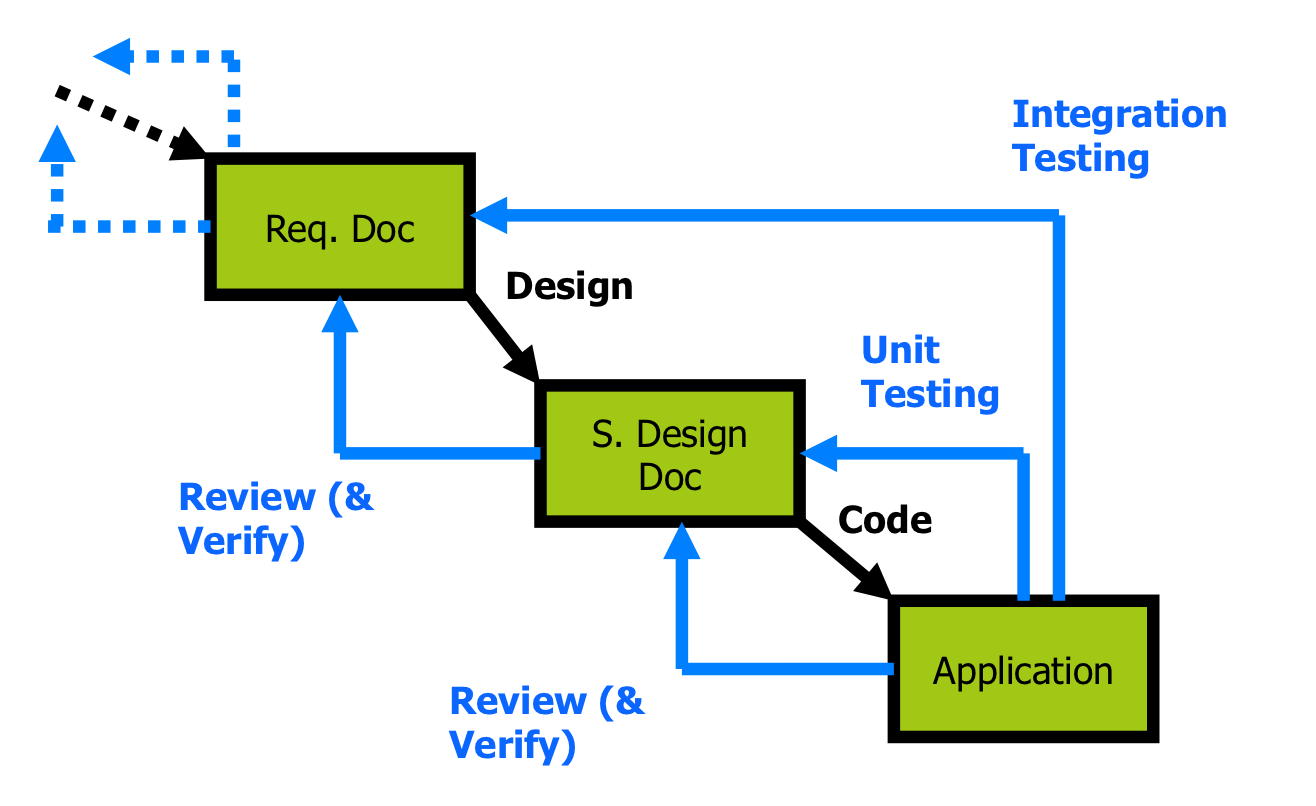
\includegraphics[scale=0.4]{SoftwareLifecycle.png}

\noindent \wss{Fill in your answer below}

\begin{enumerate}[a)]
\item Abstraction
  \begin{itemize}
  \item
  \item
  \item
  \end{itemize}
\item Separation of Concerns
  \begin{itemize}
  \item
  \item
  \item
  \end{itemize}
\end{enumerate}

%%%%%%%%%%%%%%%%%%%%%%%%%%%%%%%%%%%%%%%%%%%%%%%%%%%%%%%%%%%%%%%%%%%%%%

\newpage

\noindent Consider the specification for two modules: SeqServices and SetOfInt.

\section* {Sequence Services Library}

\subsection*{Module}

SeqServicesLibrary

\subsection* {Uses}

None

\subsection* {Syntax}

\subsubsection* {Exported Constants}

None

\subsubsection* {Exported Types}

None 

\subsubsection* {Exported Access Programs}

\begin{tabular}{| l | l | l | p{5cm} |}
\hline
\textbf{Routine name} & \textbf{In} & \textbf{Out} & \textbf{Exceptions}\\
\hline
max\_val & seq of $\mathbb{Z}$ & $\mathbb{N}$ & ValueError\\
  \hline
count & $\mathbb{Z}$, seq of $\mathbb{Z}$ & $\mathbb{N}$ & ValueError\\
\hline
spices & seq of $\mathbb{Z}$ & seq of string & ValueError\\
\hline
new\_max\_val & seq of $\mathbb{Z}$, $\mathbb{Z} \rightarrow \mathbb{B}$ &
                                                                           $\mathbb{N}$ & ValueError\\
\hline
  
\end{tabular}

\subsection* {Semantics}

\subsubsection* {State Variables}

None

\subsubsection* {State Invariant}

None

\subsubsection* {Assumptions}

\begin{itemize}
\item All access programs will have inputs provided that match the types
  given in the specification.
\end{itemize}

\subsubsection* {Access Routine Semantics}

\noindent max\_val($s$)
\begin{itemize}
\item output: $\mathit{out} := | m |: \mathbb{N} \text{ such that } (m \in s) \wedge
  \forall (x: \mathbb{Z} | x \in s : | m | \geq | x |)$
\item exception: $(|s| = 0 \Rightarrow \text{ValueError})$
\end{itemize}

\noindent count($t, s$)
\begin{itemize}
\item output: $\mathit{out} := + (x: \mathbb{Z} | x \in s \wedge x = t : 1)$
\item exception: $(|s| = 0 \Rightarrow \text{ValueError})$
\end{itemize}

\noindent spices($s$)
\begin{itemize}
\item output: $\mathit{out} := \langle x: \mathbb{Z} | x \in s : (x \leq 0
  \Rightarrow \text{``nutmeg"} | \text{True} \Rightarrow \text{``ginger"}) \rangle$
\item exception: $(|s| = 0 \Rightarrow \text{ValueError})$
\end{itemize}

\noindent new\_max\_val($s$, $f$)
\begin{itemize}
\item output: $\mathit{out} := \text{max\_val}(\langle x: \mathbb{Z} | x \in s
  \wedge f(x): x \rangle )$
\item exception: $(|s| = 0 \Rightarrow \text{ValueError})$
\end{itemize}

%%%%%%%%%%%%%%%%%%%%%%%%%%%%%%%%%%

\newpage

\section* {Set of Integers Abstract Data Type}

\subsection* {Template Module}

SetOfInt

\subsection* {Uses}

None

\subsection* {Syntax}

\subsubsection* {Exported Types}

SetOfInt = ?

\subsubsection* {Exported Constants}

None

\subsubsection* {Exported Access Programs}

\begin{tabular}{| l | l | l | p{6cm} |}
\hline
\textbf{Routine name} & \textbf{In} & \textbf{Out} & \textbf{Exceptions}\\
\hline
new SetOfInt & seq of $\mathbb{Z}$ & SetOfInt & \\
\hline
is\_member & $\mathbb{Z}$ & $\mathbb{B}$ & \\
\hline
to\_seq &  & seq of $\mathbb{Z}$ & \\
\hline
union & SetOfInt & SetOfInt & \\
\hline
diff & SetOfInt & SetOfInt & \\
\hline
size &  & $\mathbb{N}$ & \\
\hline
empty &  & $\mathbb{B}$ & \\
\hline
equals & SetOfInt & $\mathbb{B}$ & \\
\hline

\end{tabular}

\subsection* {Semantics}

\subsubsection* {State Variables}

$s$: set of $\mathbb{Z}$

\subsubsection* {State Invariant}

None

\subsubsection* {Assumptions}

\begin{itemize}
\item The SetOfInt constructor is called for each object instance before any
  other access routine is called for that object.  The constructor can only be
  called once.  All access programs will have inputs provided that match the types
  given in the specification.
\end{itemize}

\subsubsection* {Access Routine Semantics}

\noindent new SetOfInt($x_s$):
\begin{itemize}
\item transition: $s := \cup (x: \mathbb{Z} | x \in x_s : \{ x \} )$
\item output: $\mathit{out} := \mathit{self}$
\item exception: none
\end{itemize}

\noindent is\_member($x$):
\begin{itemize}
\item output: $x \in s$
\item exception: none
\end{itemize}

\noindent to\_seq():
\begin{itemize}
\item output: $out := \mbox{set\_to\_seq}(s)$
\item exception: none
\end{itemize}

\noindent union($t$):
\begin{itemize}
\item output: $\text{SetOfInt} (\mbox{set\_to\_seq}(s) ||
  t.\text{to\_seq()})$

  \textit{\# in case it is clearer, an alternate version of output is:}
  
  $\text{SetOfInt}(\text{set\_to\_seq}(s \cup \{x: \mathbb{Z} | x \in t.\text{to\_seq()} : x \}))$
  
\item exception: none
\end{itemize}

\noindent diff($t$):
\begin{itemize}
\item output:
  $\text{SetOfInt}( \text{set\_to\_seq} (s \cap \text{complement}(t.\text{to\_seq()})))$
  
\item exception: none
\end{itemize}

\noindent size():
\begin{itemize}
\item output: $| s |$
\item exception: none
\end{itemize}

\noindent empty():
\begin{itemize}
\item output: $s = \varnothing$
\item exception: none
\end{itemize}

\noindent equals($t$):
\begin{itemize}
\item output: $\forall ( x: \mathbb{Z} | x \in \mathbb{Z} : x \in
  t.\text{to\_seq()} \leftrightarrow x \in s)$ \textit{\# this means:} $t.\text{to\_seq}() = s$
\item exception: none
\end{itemize}

\subsection*{Local Functions}

\noindent $\mbox{set\_to\_seq}: \text{set of } \mathbb{Z} \rightarrow \mbox{seq of }
\mathbb{Z}$\\
\noindent
$\mbox{set\_to\_seq}(s) \equiv \langle x: \mathbb{Z} | x \in s : x \rangle$
\textit{\# Return a seq of all of the elems in the set s, order does not matter}\\

\noindent $\mbox{complement}: \text{seq of } \mathbb{Z} \rightarrow \mbox{ set of }
\mathbb{Z}$\\
$\mbox{complement}(A) \equiv \{ x: \mathbb{Z} | x \not\in A : x \}$\\

%%%%%%%%%%%%%%%%%%%%%%%%%%%%%%%%%%

\newpage

\noindent
\begin{minipage}{\textwidth}
\question{15 marks} \label{Q_PythonCode}

\wss{Complete Python code to match the above specification.}  The files you need
to complete are: \texttt{SeqServicesLibrary.py} and \texttt{SetOfInt.py}.  Two
testing files are also provided: \texttt{expt.py} and \texttt{test\_driver.py}.
The file \texttt{expt.py} is pre-populated with some simple experiments to help
you see the interface in use, and do some initial test.  You are free to add to
this file to experiment with your work, but the file itself isn't graded.  The
\texttt{test\_driver.py} is also not graded.  However, you may want to create
test cases to improve your confidence in your solution.  The stubs of the
necessary files are already available in your \texttt{src} folder.  The code
will automatically be imported into this document when the \texttt{tex} file is
compiled.  You should use the provided Makefile to test your code.  You will NOT
need to modify the Makefile.  The given Makefile will work for \texttt{make
  test}, without errors, from the initial state of your repo.  The \texttt{make
  expt} rule will also work, because all lines of code have been commented out.
Uncomment lines as you complete work on each part of the modules relevant to
those lines in \texttt{expt.py} file.  The required imports are already given in
the code.  You should not make any modifications in the provided import
statements.  You should not delete the ones that are already there.  Although
you can solve the problem without adding any imports, if your solution requires
additional imports, you can add them.  As usual, the final test is whether the
code runs on mills.

Any exceptions in the specification have names identical to the expected Python
exceptions; your code should use exactly the exception names as given in the
spec.

You do not need to worry about doxygen comments.  However, you should include
regular comments in the code where it would benefit from an explanation.

You do not need to worry about PEP8.  Adherence to PEP8 will not be part of the
grading.

Remember, your code needs to implement the given specification so that the
interface behaves as specified.  This does NOT mean that the local functions
need to all be implemented, or that the types used internally to the spec need
to be implemented exactly as given.  If you do implement any local functions,
please make them private by preceding the name with double underscores.\\

\end{minipage}

\newpage

\subsection*{Code for SeqServicesLibrary.py}

\noindent \lstinputlisting{./src/SeqServicesLibrary.py}

\newpage

\subsection*{Code for SetOfInt.py}

\noindent \lstinputlisting{./src/SetOfInt.py}

\newpage

\subsection*{Code for expt.py}

\noindent \lstinputlisting{./src/expt.py}

\newpage

\subsection*{Code for test\_driver.py}

\noindent \lstinputlisting{./src/test_driver.py}

\newpage

%%%%%%%%%%%%%%%%%%%%%%%%%%%%%%%%%%

\noindent
\begin{minipage}{\textwidth}
\question{5 marks} 

Critique the design of the interface for the SetOfInt module.  Specifically,
review the interface with respect to its consistency, essentiality, generality
and minimality.  Please be specific in your answer.

\wss{Put your answer for each quality below.}

\begin{itemize}
\item \textbf{consistency}:
\item \textbf{essentiality}:
\item \textbf{generality}:
\item \textbf{minimality}:
\end{itemize}

\end{minipage}

%%%%%%%%%%%%%%%%%%%%%%%%%%%%%%%%%%

\newpage

\noindent
\begin{minipage}{\textwidth}
\question{4 marks}

The module SetOfInt is for a set of integers.  Please answer the following
questions related to making that module generic. 
\begin{enumerate}[a.]
\item How would you change the specification to make it generic?  (Specifically
  what changes would you make to the given specification.  You don't need to
  redo the spec, just summarize what changes you would need to make.)
\item What changes would you need to make to the Python
implementation to make it generic for type T?  (Again, you can describe and
characterize the changes; you don't actually have to make them.)
\item What relational operator needs to be defined for type T to be a valid
  choice?
\item BONUS (1 mark) How would you specify (in the MIS) the relational operator
  constraint (from the previous question) on the generic type T?
\end{enumerate}

\wss{Put your answer below.}

\begin{enumerate}[a.]
\item
\item
\item
\item (BONUS)
\end{enumerate}

\end{minipage}

\end{document}